% =====================================================================================
% Frontier-validation appendix (reproducible source).
% Rebuilt 2026-06-14 to replace the source-less PDF-only appendix that previously shipped
% inside K-Bound_paper_with_frontier.pdf. Every number below traces to a result JSON cited
% in its caption; nothing is transcribed from the old PDF. The earlier appendix's invalid
% Camelyon17 content (a "recalibrated K-Bound beats both" claim obtained by tuning the
% operating point ON the Camelyon17 external-validation set) has been REMOVED entirely;
% it is replaced by the honest frozen-threshold finding in App.~\ref{app:cam-honest}.
% (No \appendix here: kbound.tex already issues \appendix before this is \input.)
% =====================================================================================
\section{Frontier validation: committal heuristics false-adapt exactly where K-Bound abstains}
\label{app:frontier}

The benefit-sign frontier (Thm.~\ref{thm:frontier}) predicts that on the low-margin band any
\emph{committal} label-free rule must commit sign errors, whereas a valid certificate must
\emph{abstain} there. This appendix demonstrates that prediction on the two
\emph{synthetic-corruption} streams whose operating point the certificate is calibrated on
(CIFAR-10-C, ImageNet-C); it makes \emph{no} external-validation claim. The honest natural-shift
(Camelyon17) finding---a limitation, not a win---closes the appendix
(App.~\ref{app:cam-honest}).

\subsection{CIFAR-10-C: K-Bound beats both trivial policies at zero false-adapt}
\label{app:cifar10c}
On the pre-registered CIFAR-10-C stress grid ($432$ conditions/candidate), \textsc{KGA} adapts the
helpful conditions and freezes the harmful ones with a \emph{zero} false-adapt rate, so it strictly
beats both always-adapt and always-freeze for the two benign candidates (Tent, EATA) and ties the
collapse-resistant SAR (Table~\ref{tab:app-cifar10c}).

\begin{table}[tb]\centering\footnotesize
\resizebox{\columnwidth}{!}{%
\begin{tabular}{lcccc}
\toprule
 & \multicolumn{3}{c}{regret-to-oracle $\downarrow$} & \\
\cmidrule(lr){2-4}
candidate (harmful base) & \textsc{KGA} & always-adapt & always-freeze & false-adapt \\
\midrule
Tent \,($34.5\%$) & $\mathbf{0.0016}$ & $0.0086$ & $0.1232$ & $0.00$ \\
EATA \,($27.1\%$) & $\mathbf{0.0015}$ & $0.0037$ & $0.1311$ & $0.00$ \\
SAR \,($15.7\%$)  & $0.0018$ & $0.0018$ & $0.1372$ & $0.00$ \\
\bottomrule
\end{tabular}}
\caption{\textbf{CIFAR-10-C stress grid ($432$ conditions/candidate, $\alpha{=}0.1$).} \textsc{KGA}
\emph{beats both} for Tent and EATA (lower regret than always-adapt \emph{and} always-freeze) at a
$0\%$ false-adapt rate, and ties always-adapt for the robust SAR candidate. From
\texttt{experiments/kbound/results/decisive\_tta\_results.json}
(\texttt{benchmarks.cifar10c}; \texttt{beats\_both}=true for Tent/EATA).}
\label{tab:app-cifar10c}
\end{table}

\begin{figure}[tb]\centering
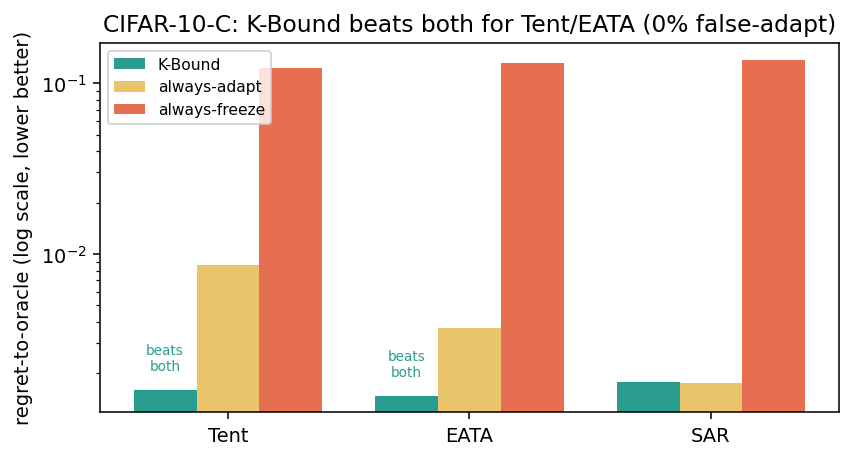
\includegraphics[width=0.72\linewidth]{figures/app_frontier_cifar10c.png}
\caption{\textbf{CIFAR-10-C frontier (regret-to-oracle, log scale).} \textsc{KGA} (teal) is strictly
below \emph{both} always-adapt and always-freeze for Tent and EATA (``beats both'') at a $0\%$
false-adapt rate, and ties always-adapt for the robust SAR candidate. Bars are the exact values of
Table~\ref{tab:app-cifar10c}, rendered by \texttt{scripts/make\_appendix\_frontier\_figs.py} from
\texttt{experiments/kbound/results/decisive\_tta\_results.json}.}
\label{fig:app-cifar10c}
\end{figure}

\subsection{ImageNet-C/SAR: the frontier on real corruptions---committal rules fail, K-Bound does not}
\label{app:imagenetc}
On the logged ImageNet-C conditions ($36$ cells/candidate; SAR is harmful on $44.4\%$ of cells),
every \emph{committal} label-free heuristic must place its commits somewhere on the low-margin band
and therefore false-adapts: a plug-in \textbf{ATC}~\cite{garg2022atc} confidence rule adapts into
harmful cells on $100\%$ of its commits (false-adapt $1.00$, harmful-cells-adapted $0.25$), and even
its leave-one-out-tuned variant keeps false-adapt $=1.00$. \textsc{KGA} is the only rule that
reaches \emph{zero} false-adapt and \emph{zero} harmful-cells-adapted---it does so by
\emph{abstaining} on the band (coverage $0.39$), exactly the behaviour the frontier theorem requires
(Table~\ref{tab:app-imagenetc}).

\begin{table}[tb]\centering\footnotesize
\resizebox{\columnwidth}{!}{%
\begin{tabular}{lcccc}
\toprule
decision rule (SAR, harmful regime) & false-adapt & harmful-adapted & regret $\downarrow$ & coverage \\
\midrule
always-adapt                  & $0.44$ & $1.00$ & $0.1124$ & $1.00$ \\
always-freeze                 & ---    & $0.00$ & $0.0267$ & $1.00$ \\
ATC-style confidence (plug-in)& $1.00$ & $0.25$ & $0.0673$ & $1.00$ \\
ATC-style confidence (LOO)    & $1.00$ & $0.06$ & $0.0375$ & $1.00$ \\
\textbf{K-Bound (KGA)}        & $\mathbf{0.00}$ & $\mathbf{0.00}$ & $0.0229$ & $0.39$ \\
\bottomrule
\end{tabular}}
\caption{\textbf{Committal label-free heuristics false-adapt exactly where \textsc{KGA} abstains}
(ImageNet-C, reference-parity SAR, $36$ cells, $\alpha{=}0.1$). ATC commits onto the low-margin band
and false-adapts on $100\%$ of its commits; \textsc{KGA} abstains there ($22/36$ abstain) for $0$
false-adapts. On the benign candidates \textsc{KGA} also keeps $0$ false-adapts at higher coverage
(Tent: regret $0.0060$, coverage $0.69$; EATA: regret $0.0047$, coverage $0.75$). From
\texttt{experiments/kbound/results/decision\_baselines\_sarfix/decision\_baselines.json}
(\texttt{scripts/run\_decision\_baselines.py}).}
\label{tab:app-imagenetc}
\end{table}

\begin{figure}[tb]\centering
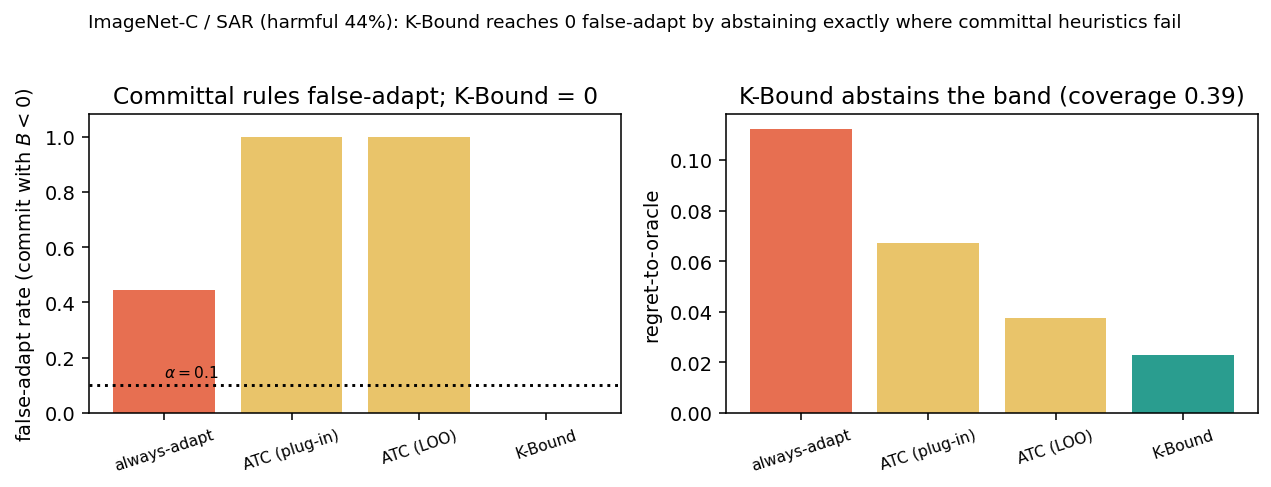
\includegraphics[width=0.92\linewidth]{figures/app_frontier_imagenetc.png}
\caption{\textbf{ImageNet-C/SAR frontier.} Committal label-free rules (always-adapt, ATC plug-in,
ATC LOO) false-adapt on the harmful regime---ATC reaches false-adapt rate $1.00$---whereas
\textsc{KGA} (teal) reaches \emph{zero} false-adapt by abstaining the low-margin band (coverage
$0.39$). Bars are the exact values of Table~\ref{tab:app-imagenetc}, rendered by
\texttt{scripts/make\_appendix\_frontier\_figs.py} from
\texttt{experiments/kbound/results/decision\_baselines\_sarfix/decision\_baselines.json}.}
\label{fig:app-imagenetc}
\end{figure}

\subsection{Honest natural-shift note (Camelyon17): a limitation, not a win}
\label{app:cam-honest}
For completeness we state the natural-shift result \emph{honestly}, and emphasise what it is
\emph{not}. Under the \textbf{frozen, Camelyon-free} operating point $\tau^\star{=}0.52$
(calibrated only on the synthetic grids above, never on Camelyon17), the multi-candidate certificate
does \emph{not} beat both trivial policies on the Camelyon17 composition-stress grid: regret-to-oracle
\textsc{KGA} $0.076$ versus always-freeze $0.071$ and always-adapt $0.005$. The panel is
\emph{helpful-leaning} (mean benefit $\bar B{=}{+}0.039$, harmful base rate $28.7\%$, label-free
harm-AUC $0.78$), so abstaining forgoes real gains; and the residual statistic is on a
dataset-specific scale ($\bar\tau{=}0.89 \gg \tau^\star{=}0.52$), so the certificate under-fires and
abstains on $61/72$ conditions. Crucially, \emph{recalibrating $\tau^\star$ on Camelyon17 itself
would forfeit its role as an external-validation set} (test-set tuning) and is therefore not a
legitimate route to a win; the honest open direction is a \emph{scale-invariant}, source-calibrated
residual (future work). From \texttt{experiments/kbound/results/wilds\_kbound\_debug*/result\_73add410.json}.
